\subsection{Community detection}

In this PhD project there are two different school of thoughts explored for community detection: modularity maximisation and generative models. The first finds communities (or modules or blocks) into the network by maximising the separation between the communities which is measured by a cost function see Eq \ref{}. This is usually done by moving the nodes between communities until the function converges. In the literature there were several mathematical functions proposed to maximise the modularity of the graph such as FastUnfold \citet{Blondel2008-ik} (also known as Louvain and it initially used in PGCNA), Constant Pots Model (CPM or Leiden \citet{Traag2019-ne}, improvement from Louvain), InfoMap \citet{Rosvall2008-kw} etc. This suite of algorithms usually requires a parameter (e.g. resolution parameter) to guide the models to the range of communities. A well-known problem with Modularity Maximisation is the resolution-limit problem where after a certain threshold, the \textbf{algorithm spits out non-sense. }

The second class of community detection algorithms is represented by Stochastic Block Models (SBM) and these work by generating different networks with different partitions by fitting the observed network. SBMs were first introduced in the 80's to social networks \citet{Holland1983-oo} but become more popularised in 2010 with the work of \citet{Karrer2011-si} and more recently by the Tiago Peixoto. The new models introduced by Peixoto are non-parametric, that is they do not need any parameter to adjust the algorithm to find more or less communities. The breakthrough that the Peixoto did in his work was to use a metric called minimum description length to quantify the information present through the communities in the network. In addition, by using generative approach, i.e. generating blocks, it looks at different way to compress the data. Thus, finding communities is about compressing information. With these two notions the Peixoto proposes new algorithms to detect communities and not only that, but also to measure the performance of the algorithms. This is crucial in applications such as in this project, where it is very hard to quantify \& measure the progress. Lastly, in his work Peixoto stresses out the fact there SBM are good general models and that in a network without the ground truth there might be a chance of the community detection algorithms not to find all the communities. This is illustrated in Figure (… ) 

This part of the literature review is structure so that it offers an overview of Leiden and Louivan, representing the mainstream approach to community detection. This is followed by the criticism and limitation of these models. Lastly, the alternative is presented which comes through the SBM Models.


% Leiden and others
\subsubsection{Modularity maximisation}

Leiden and Louvain \citet{Traag2019-ne,Blondel2008-ik} are relatively simple algorithms with a similar strategy as in the agglomerative hierarchical clustering, where each node (gene) has its own partition, then these are moved until the optimal partitions is found. The optimal is usually asses by Eq \ref{}, which is called modularity function. The resolution parameter controls the number of communities, lower values gives less communities where higher lead to more. An alternative to the Modularity maximisation is Constant Pots Model (CPM) introduced by \citet{Traag2011-if}. Both functions are explored in this project see Section \ref{}.

\citet{Traag2019-ne} addresses the above Louivan's limitation  which it founds arbitrarily badly connected communities and resolution limit. The latter refers that Louivan is not able to find more than $\sqrt{2E}$, where E is the total number of edges and as shown in \citet{Peixoto2021-jx}, it can not find smaller communities even when there is a statistical evidence for it. Leiden is a culmination of other efforts to improve Louivan\cite{Ozaki2016-dl,Waltman2013-zw,Bae2017-rz, Traag2015-tq} and the authros prove and guarantee that the algorithm converges to stable partitions, no disconnected communities and it shows that it is faster. Disconnected communities is something that was observed by \citet{Care2019-ij} when they used Louivan algorithm and set the number of edges per gene smaller than 2. Thus, it is an improvement to the original algorithm.

% Comparative studies
The work of \citet{Shemirani2023-ww} is used to find short-segment shared by a group of people who are distantly related, with goal to find rare traits and disease in biobanks. For these kind of applications, community detection algorithms are used and the authors compare multiple popular methods Leiden, Louivan, InfoMap \citet{Rosvall2008-kw} and Markov Clustering (MCL) \citet{Van_Dongen2008-yj}. Despite being a different problem from the one addressed in this PhD, the work of \citet{Shemirani2023-ww} is relevant as it offers a comparison between the different community detection algorithms. Leiden and Louivan generally have higher Modularity scores but The MCL and InfoMap are closer to the ground-truth communities. The authors reason that is due to the resolution limit and the Leiden, Louivan are not able to find smaller communities. This reinforces, the problem described above and raised by Tiago \citet{Peixoto2021-jx} and others \cite{Fortunato2007-gh, Traag2019-ne}, covered in the next section (\ref{s:lit:descriptive_inference}).

% Critiques for Leiden
\subsubsection{Descriptive vs Inference} \label{s:lit:descriptive_inference}

In the \textit{"Descriptive vs. Inferential Community Detection in Networks"} \citet{Peixoto2021-jx}, the author shows the limitation of using the modularisation based algorithms to find communities which are also called descriptive methods. The gist of the study is that the descriptive methods such as modularity maximisation looks for the patterns in the network even when there are not there; thus, finding communities in a random generated network. Generative or infer methods such as SBM are immune to this and will not find any communities. 

The major flow of the modularity maximisation based models such as Leiden or Louivan that these do not take in account the observed network\footnote{In the context of the PhD, is the co-expressed network generated from correlation measurements.} from the null-model\footnote{A network with the same properties as the one observed; i.e. may refer to the degree distribution, how nodes are connected inside the community etc.} this is due to lack of incorporating the optimisation step in assessing the performance of the algorithm; i.e. cost function. In this paper \citet{Peixoto2021-jx} demonstrates and shows in detail the problem, but it was also recognised earlier \citet{Guimera2004-gv}.

While the study in 2021 \citet{Peixoto2021-jx} compares the two algorithm classes more at the theoretical and foundational levels, with occasional direct comparison of the number of communities discovered by each method. In 2023 \citet{Peixoto2023-rt}, the authors overcome the technical challenge of comparing the two community detection algorithms and it introduces description length as common metric. This is a metric derived from information theory which quantifies the information in a network through the use of entropy. The main takeaway of \citet{Peixoto2023-rt} is that the authors in this paper demonstrated that the modularity maximisation methods are a special case of generative models and that these can be compared.

% In this paper \citet{Peixoto2021-jx}, chapter Tiago presents the differences between the descriptive and inference models. The former, tries to find patterns in a given network and it does not account for the rules that the network was made. While,  inference models are trying to generate the partitions which are responsible for the formation of the observed network. The author argues that descriptive models are not suitable for inference problems; i.e. some sort of knowledge is inferred from the network, trying to ask why questions, such as data analysis problems. While inference networks are more robust and suitable for this kind of problems.

% SBM
\subsubsection{A generative approach}


Stochastic Block Model (SBM) are generating partitions that best explain the observed network (i.e. generated from co-expressed networks). One should imagine that the observed network can be reconstructed from different network blocks and the challenge is given by finding these partitions. This is  different from the Leiden or Louivan methods which shuffle nodes around until the partitions are found that describe the best the given network. 

\begin{figure}[!htb]    
    \centering
    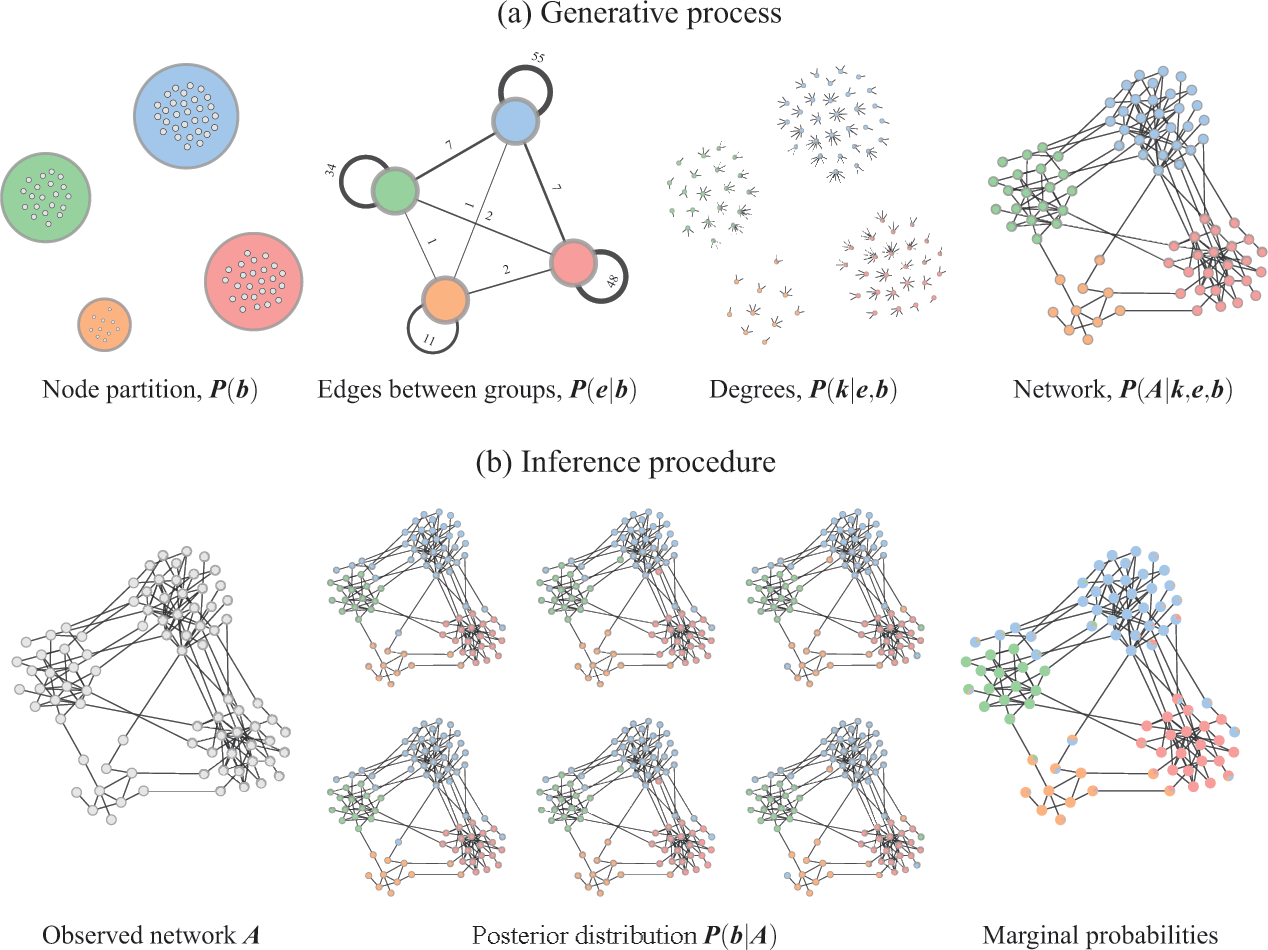
\includegraphics[width=1.0\textwidth,height=1.0\textheight,keepaspectratio]{Sections/Network_I/Resources/dc-sbm_explained.png}
    \caption{SBM explained. This is Figure 3 from \citet{Peixoto2021-jx}}
    \label{fig:N_I:dc-sbm_explained}
\end{figure}


There is a good description of the degree corrected SBM version in Figure \ref{fig:N_I:dc-sbm_explained} which is a special type of SBM that accounts for the nodes' degree. For a node partition, $P(B)$ the network may be divided into 4 different communities. Each of these communities will have nodes that are connected inside (in-degree) or/and outside of the partition (out-degree); this is given by $P(e|b)$, where e is a matrix that specify how many edges go between groups r and s. Then, inside of each module, it can be looked at the individual nodes and their connections (degree), which is given by $ P(k|e,b)$; in the network before last it can be seen the un-connected nodes which are known as “stubs” or “half-edges”. With all this information, the nodes are connected and formed the observed network. Different partitions are generated and chosen the ones which held the best results according to the minimum description length.

\begin{equation} \label{eq:sbm}
         P(b|A) = \frac{P(A|b)P(b)}{P(A)}
\end{equation}

How well the partition b represent the network is measured by the description length, which is using concepts from Information Theory; i.e. how much information is needed to describe the network through likes of entropy. Lower information means is desired as the network is more ordered; i.e. that more ‘rules’ that generally describes the trends in the graph. More information needed, means that  when reconstructing the graph we need more information to do that; i.e. more connections, larger the entropy. As it expected, for more communities there is a need for more information to describe the network. The author noted that this process is very similar to information compression.

Compared to the other algorithms SBM are more complex and more computational taxing. However, based on the experience in this project, the computational time is not as high as the one from iCluster\citet{Mo2013-zi}. In addition, the standard SBM \citet{Peixoto2019-fg, Peixoto2017-gc, Peixoto2017-ua, Karrer2011-si} have their own limitation in terms of how many communities can they found, which is limited at $\sqrt{N}$, where $N$ is the number of nodes. In \citet{Peixoto2014-yb} this issue is addressed by proposing a hierarchical Stochastic Block Model (hSBM). The central idea is to re-apply SBM once the limit of partitions is found, thus increasing the number of partitions found. This also comes to an additional computational cost.

% Summary
\subsubsection{Summary}


Leiden and Louivan are widely applied to biological problems, only through the lens of PGCNA both were applied to subtyping of the breast, lung and glioblastoma cancer cohorts from TCGA \cite{Tanner2023-wa, Care2019-ij}. In all of these applications, community detection serve a key role in selecting and inferring biological meaning from the networks. Thus, the serious limitations raised \citet{Peixoto2021-jx,Guimera2004-gv, Peixoto2023-rt} poise a serious challenge to the applicability of Leiden and Louivan in disease subtyping, and in fact in any biological networks. 


All Leiden, Louivan and SBM have their own library packages\footnote{Leiden - \url{https://leidenalg.readthedocs.io/en/stable/intro.html}, Louivan - \url{https://python-louvain.readthedocs.io/en/latest/}, SBM - \url{https://graph-tool.skewed.de/}} which are available online. However, SBM's library is by far the most maintained, advanced and complete out of the others. 

To sum it up, both classes of algorithms are applied to a wide range of applications in biology and are available to use. The main difference is that the Leiden, Louivan may generate 'spurious' communities and it will run faster, but SBM family will be slower but closer to the ground truth.




